\subsection*{Resultater}
Resultater har en boundary. Til denne er der opstillet en controlklasse. Boundary og tilhørende controller fremgår af \autoref{fig:MVCresultater}. 

\begin{figure} [H]
\centering
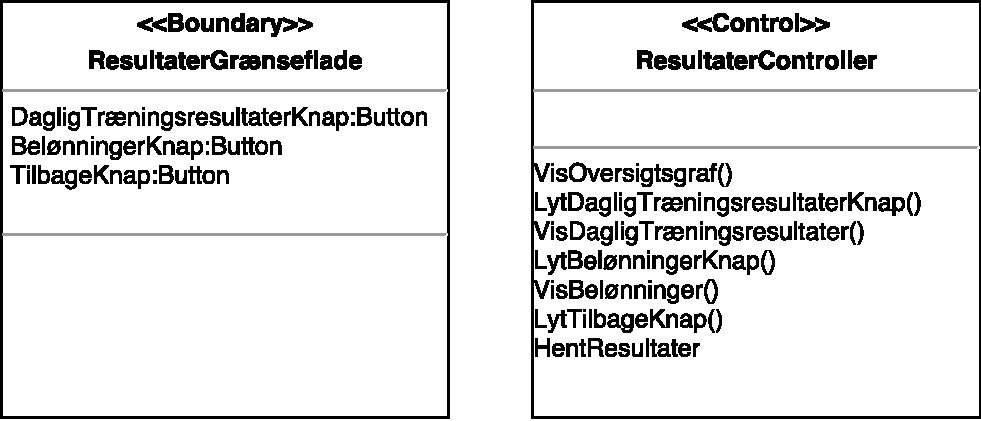
\includegraphics[width=0.8\textwidth]{figures/MVC/Resultater}
\caption{Designklasser for resultater}
\label{fig:MVCresultater}
\end{figure}

\noindent
I \textit{ResultaterGrænseflade} er der opstillet tekstfelt og knapper. Disse er af typen TextView og Button. Derudover er der Graf og Tabel til at visualisere resultaterne. \textit{OBS!! Dette er stadig lidt uklart}. 
Controlleren for \textit{Resultater} indeholder Hent, Vis og Lyt metoder. 

I sammenspil med designklasserne for resultater er der udarbejdet et sekvensdiagram, hvilket fremgår af \autoref{fig:SEKResultater}

\begin{figure} [H]
\centering
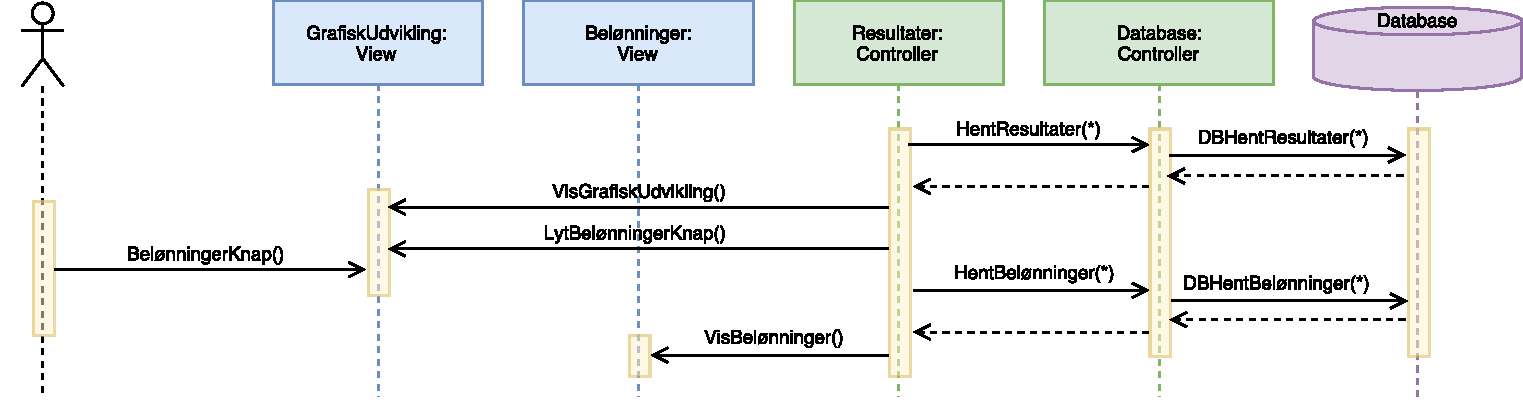
\includegraphics[width=1\textwidth]{figures/Sek/SEKResultater}
\caption{Sekvensdiagram for Resultater.}
\label{fig:SEKResultater}
\end{figure} 

\noindent 
Controlleren, \textit{Resultater} henter fra resultater fra modellen \textit{KonditionResultater}, denne er yderligere beskrevet i \autoref{sec:entity}. Grænsefladen \textit{Resultater} viser UgentligeResultater i en graf. Brugeren har mulighed for at trykke KalenderKnap eller BeløningerKnap. Trykker brugeren på KalenderKnap vises en kalender i grænsefladen, hvor brugeren har mulighed for at vælge en dag. Vælges dette vises resultater i en graf for den valgte dag. Vælger brugeren at trykke på BeløningerKnap vises en tabel med beløninger. Trykker brugeren ikke på en af knapperne vises grafen med UgentligeResultater.  
 
%Der er til \textit{ResultaterGrænseflade} opstillet en \textit{ResultatController}, der har til formål at hente nye resultater fra dagens træning i træningscontrolleren, når resultater tilgås via hovedmenugrænsefladen. Herefter vises en oversigtsgraf over udført træning. Træningscontrolleren fremgår af \autoref{fig:MVCTraening}.
%Controlleren lytter på om brugeren trykker på de angivne knapper i grænsefladen for resultater og viser valgt handling, hvis dette er tilfældet. 
